% \documentclass{minimal}
% \usepackage{tikz}

% \begin{document}
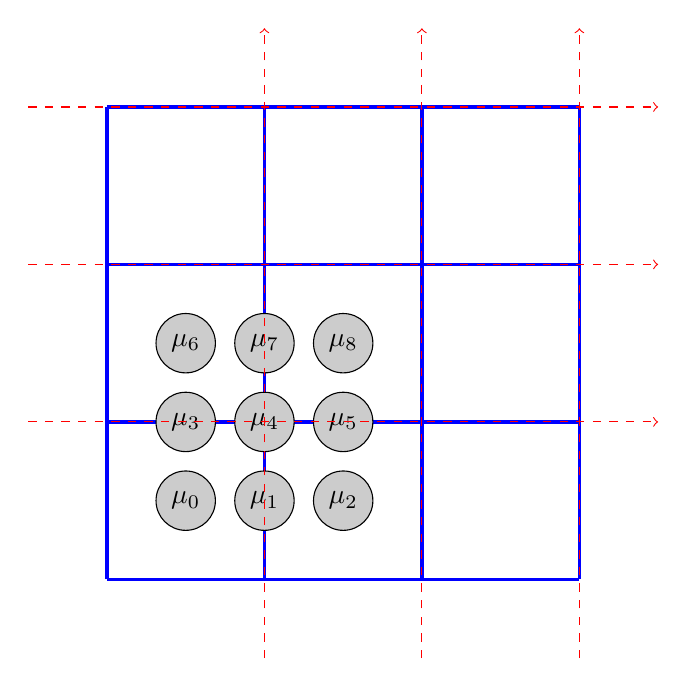
\begin{tikzpicture}[darkstyle/.style={circle,draw,fill=gray!40,minimum size=20}]

    \newcommand*{\cellsize}{2}%
    \newcommand*{\numcells}{3}%
    \newcommand*{\arrowoffset}{(1/2)}%

    \draw [step=\cellsize, blue, very thick] (0,0) grid ({\cellsize*\numcells},{\cellsize*\numcells});


  \foreach \x in {0,...,2}
  \foreach \y in {0,...,2}
  {\pgfmathtruncatemacro{\label}{\numcells * \y + \x}
       \node [darkstyle]  (\x\y) at ({\x + \cellsize / 2},{\y + \cellsize / 2}) {$\mu_{\label}$};}


    % horizontal ↓
    \foreach \i in {0,...,2}
        \draw[red, dashed, ->] ({-\arrowoffset * \cellsize}, {(\i + \cellsize/2) * \cellsize})
        -- ({(\numcells + \arrowoffset) * \cellsize}, {(\i + \cellsize/2) * \cellsize}) ;

    % vertikal ↓
    \foreach \i in {0,...,2}
        \draw[red, dashed, ->] ({(\i + \cellsize/2) * \cellsize}, {-\arrowoffset * \cellsize})
        -- ({(\i + \cellsize/2) * \cellsize}, {(\numcells + \arrowoffset) * \cellsize}) ;

    % % diagonal ↓
    % \foreach \i in {0,...,2}
    %     % \draw[red, dashed, ->] ({-\arrowoffset * \cellsize}, {(\i - \cellsize/2) * \cellsize})
    %     % -- ({(\numcells + \arrowoffset) * \cellsize}, {(\numcells + \i - \cellsize/2) * \cellsize}) ;
    %     \draw[red, dashed, ->] (0, {(\i - \cellsize) * \cellsize})
    %     -- ({(\numcells) * \cellsize}, {(\numcells + \i - \cellsize) * \cellsize}) ;

    % \foreach \i in {0,...,2}
    %     \draw[red, dashed] (0,{-2 * \cellsize + \i})--({3 * \cellsize},{1 * \cellsize + \i}) ;


%   \foreach \x in {0,...,\numcells}
%     \foreach \y [count=\yi] in {0,...,\numcells}
%       \draw (\x\y)--(\x\yi) (\y\x)--(\yi\x) ;

\end{tikzpicture}
% \end{document}
